% !TeX root = 场论与凝聚态.tex

The ``microscopic free energy''\footnote{The Mellin transformation of $F$ of variable $\beta$.} will be modified to
\begin{figure}[h]
    \centering
    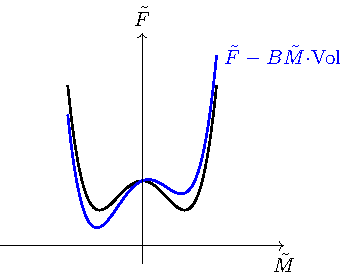
\includegraphics{figures/free_energy_in_external_field.pdf}
    \caption{free energy in external field}
\end{figure}
\begin{equation}
  \tilde{F} = \tilde{F} - B \tilde{M} \cdot \text{Vol}.
\end{equation}
and we have 
\begin{equation}
    \mathcal{Z}\left( B \right)  = \mathrm{e}^{- \frac{F\left( B \right)}{T}} = \int_{-\infty}^{\infty} \mathrm{d}\tilde{M} \, \mathrm{e}^{-\frac{1}{T} \left( \tilde{F} - B \tilde{M} \cdot \text{Vol} \right) } ,
\end{equation}
which is dominated by the double well in $\tilde{F}$.
Meanwhile, we have the relation
\begin{equation}
    M = \frac{1}{\text{Vol}} \frac{\partial F}{\partial B} = \frac{1}{\mathcal{Z}} \frac{\partial \mathcal{Z}}{\partial B} = \left< \tilde{M} \right> 
\end{equation}
and
\begin{equation}
  \chi = \frac{\partial M}{\partial B} = \frac{1}{\mathcal{Z}} \frac{\partial^2 \mathcal{Z}}{\partial B^2} - \frac{1}{\mathcal{Z}^{2}} \frac{\partial \mathcal{Z}}{\partial B} \frac{\partial \mathcal{Z}}{\partial B} = \left< M^{2} \right> - \left< M \right>^{2}
\end{equation}
It can be seen that there's some relation between long range correlation and spontaneous symmetry broken.

\subsection{Long Range Correlation and SSB in Ising Model}

The Hamiltonian of this model is
\begin{equation}
  \begin{gathered}
  H_{\text{classical}} = \sum_{\text{link $l=\langle v\,v' \rangle$}} (-J) \sigma _{v}^{z} \sigma _{v'}^{z}
  \\
  H_{\text{quantum}} = \sum_{\text{vertex $v$}} (-h) \sigma _{v}^{x}+ H_{\text{classical}}
  \end{gathered}
\end{equation}
in which $h$ and $-h$ are equivalent for the $\mathbb{Z}_2$ global symmetry. The corresponding flip operator is
\begin{equation}
  \prod{v} \sigma _{v}^{x}. \quad \text{(one for each part of the space)}
\end{equation}
Note that we doesn't need to flip all spins as our basis spacetime may consist separate parts which do not interact with each other.
The $\mathbb{Z}_2$ symmetry broken term in this model would be $- \sum_{v} B \sigma _{v}^{z}$, and our order parameter is $\sigma _{v}^{z}$.
\begin{itemize}
  \item $H_{\text{quantum}}$ in $d+1$ spacetime can b mapped to $H_{\text{classical}}$ in $d'=d+1$ space, but anisotropic $\tilde{J}_{d}\neq \tilde{J}_{\tau }$.
\end{itemize}

Now let us investigate this system through its partition function
\begin{equation}
  \mathcal{Z} = \left( \prod{v} \sum_{x=\pm 1}  \right)\mathrm{e}^{-\frac{E}{T}}
\end{equation}
where $E = \sum_{l} (-J) s_v s_{v'} - \sum_{v} B_v s_v$. 

Derivations of $\mathcal{Z}$'s logarithm gives statistic observables
\begin{equation}
  M = \frac{1}{\text{Vol}} \frac{\partial F}{\partial B} = \frac{\left( \prod_{v} \sum_{s_v = \pm 1}  \right) s_{v_0} \mathrm{e}^{-\frac{E}{T}}}{\mathcal{Z}} = \langle s_{u_0}\rangle
\end{equation}
and
\begin{equation}
  \begin{aligned}
    \chi = \left. \frac{\partial M}{\partial B} \right|_{B=0} 
    & = \frac{1}{T} \sum_{v_1} \left( \langle s_{v_0} s_{v_1} \rangle - \langle s_{v_0}\rangle \langle s_{v_1}\rangle \right)_{B=0} \\
    & = \frac{1}{T} \sum_{v_1} \langle s_{v_0} s_{v_1}\rangle
  \end{aligned}
\end{equation}
The relation above gives two cases:
\begin{itemize}
  \item if $\left< s_{v_0} s_{v_1} \right> \sim \mathrm{e}^{- \# r}$, $\chi$ is finite, and no SSB, which corresponds to high $T$ and $d \le 1$.
  \item if $\left< s_{v_0} s_{v_1} \right> \sim \text{constant}$, $\chi$ is infinite, SSB, which corresponds to low $T$ and $d \ge 2$.
\end{itemize}

\subsection{Expansion of $\mathcal{Z}$ in Low and High $T$}

An useful observation is given as
\begin{equation}
  \mathrm{e}^{\frac{J}{T} s_{v} s_{v'}} = \mathrm{e}^{\frac{J}{T}} \left( \delta_{s_v, s_{v'}} + \mathrm{e}^{-\frac{2J}{T}} \delta_{s_{v}, -s_{v'}} \right) = \cosh \frac{J}{T} \left( 1+ \tanh \frac{J}{T} s_{v} s_{v'} \right)
\end{equation}

\begin{figure}[ht]
    \centering
    \incfig{expansion-of-ising}
    \caption{Expansion of ising}
    \label{fig:expansion-of-ising}
\end{figure}

The overall factor only contributes a constant shift of Hamiltonian density, what we focus now would be the latter term of each expression.

\subsubsection{Low $T$ Expansion}
We can obtain from above that
\begin{equation}
  \mathcal{Z} = \left( \prod_{v} \sum_{s_{v} = \pm 1}  \right) \left( \prod_{l = \left< v,v' \right>}  \mathrm{e}^{\frac{J}{T}} \left( \delta_{s_v, s_{v'}} + \mathrm{e}^{-\frac{2J}{T}} \delta_{s_{v}, -s_{v'}} \right) \right).
\end{equation}
Expanding the $\displaystyle \prod $ in partition function, we will be expected to arrive at a huge product of $\delta_{s_v, s_{v'}}$ and $\delta_{s_v, - s_{v'}}$. After summing over all possible field configuration, we can match each field config with a diagram, by coloring each link where $\delta_{s_v, -s_{v'}} = 1$.

\begin{figure}[ht]
    \centering
    \incfig{domain-wall}
    \caption{Domain wall}
    \label{fig:domain-wall}
\end{figure}

\begin{equation}
  \mathcal{Z} = \sum_{\text{domain config}} \left( \mathrm{e}^{- 2J /T}  \right)^{\# \text{ of links on domain wall}} \underbrace{\left( \mathrm{e}^{J / T} \right)^{\# \text{ of links}}}_{\text{constant}}
\end{equation}
Each place between $v_0$ and $v_1$ is a possible position for domain wall to appear, thus we could write
\begin{equation}
  \# \text{ of possibilities} \sim \Bigl( \mathcal{O} (1)  \Bigr)^{\left| r \right|}.
\end{equation}
Given that entropy is logarithm of number of microstates, we discover that a new domain wall gives out a shift of free energy satisfying
\begin{equation}
  \mathrm{e}^{- \frac{\Delta F}{T} } \sim \left( \mathrm{e}^{- 2J / T} \right)^{l} \Bigl( \mathcal{O} (1)  \Bigr)^{\left| r \right|}
\end{equation}

In long-range correlation, both $l$ and $r$ scale with system size\footnote{
  For $1$-dim, $l=1$, no SSB
}, thus $\mathrm{e}^{- \Delta F / T}$ will be extremely small, revealing that it is unlikely to form domain wall in large scale, thus
\begin{equation}
  \left< s_{v_0} s_{v_1} \right> \sim  \text{constant}
\end{equation}

\subsubsection{High $T$ Expansion}
Re-write the partition function as
\begin{equation}
  \mathcal{Z} = \left( \prod_{v} \sum_{s_{v}=\pm 1}  \right)\left( \prod_{l = \left< v,v' \right>} \cosh \frac{J}{T} \left( 1+ \tanh \frac{J}{T} s_v s_{v'} \right) \right).
\end{equation}
Similarly, expanding the product in the second parenthesis, $\mathcal{Z}$ now is a polynomial of $s_v s_{v'}$ to be summed over all config. Now we denote each $s_{v} s_{v'}$ as a colored link.

After $\sum_{s_v =\pm 1} $, all monomials containing odd power of $s_v$ become zero. The remaining terms can be regarded as summation of all closed loops,
\begin{equation}
  \mathcal{Z} = \sum_{\text{closed loops}}  \left( \tanh \frac{J}{T} \right)^{\left| \text{length of loop} \right|} \cdot 2^{\left| \# \text{ of vertices} \right|} \cdot \left( \cosh \frac{J}{T} \right) ^{\left| \# \text{ of links} \right|}
\end{equation}

Now we insert $s_{v_0} s_{v_1}$ into the path integral to obtain $\left< s_{v_0} s_{v_1} \right>$. The discussion above is still compatible, however, the only difference is at the vertices of $v_0$ and $v_1$, where the original monomial with odd power of $s_{v_0}, s_{v_1}$ will remain. 

Now it's easy to see that in high temperature, the partition function is dominated by the shortest line between $v_0$ and $v_1$. Any extra deformation of the line would contribute a free energy of
\begin{equation}
  \mathrm{e}^{- \frac{\Delta F}{T}} \sim \mathcal{O}(1) \cdot \left( \tanh \frac{J}{T} \right)^{\Delta l} \ll  1
\end{equation}
when $T$ is high, any deformation is unlikely, thus
\begin{equation}
  \left< s_{v_0} s_{v_1} \right> \sim \left( \tanh \frac{J}{T} \right)^{r}
\end{equation}
